\begin{answer}
    \begin{figure}[H]
        \centering
        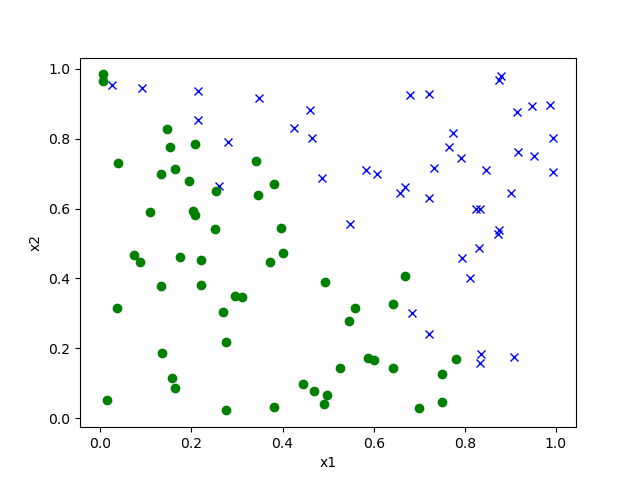
\includegraphics[width=0.75\textwidth]{../src/stability/ds1_a.png}
        \caption{Dataset A}
        \label{fig:ds1-a}
    \end{figure}
    \begin{figure}[H]
        \centering
        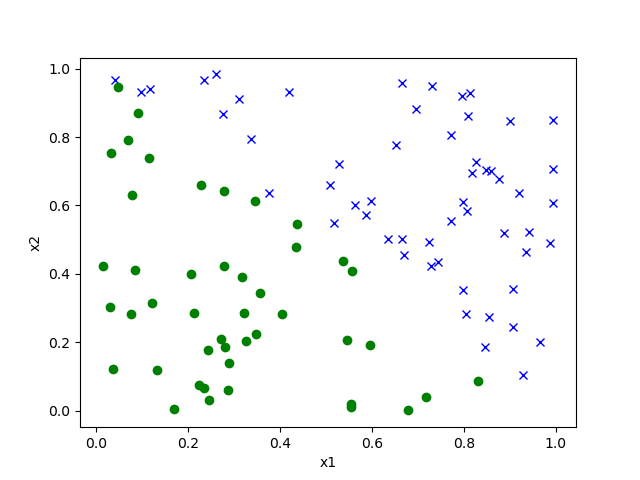
\includegraphics[width=0.75\textwidth]{../src/stability/ds1_b.png}
        \caption{Dataset B}
        \label{fig:ds1-b}
    \end{figure}
    Plotting the two datasets, we can see that dataset A have interleaving
    points between two classes while B seem to have a clear boundary between
    two classes. It may be that the gradient of loss to theta is never going
    to be zero for dataset B, so the model is not converging. We can always 
    increase theta to make the loss smaller, but it will never reach the minimum.
\end{answer}
